\chapter{Opis projektnog zadatka}
		
		\text Cilj ovog projekta razviti je programsku podršku za web aplikaciju \textit{Ozdravi} koja će korisnicima omogućiti olakšanu komunikaciju s pedijatrom i liječnikom obiteljske medicine, te lakši pregled podataka o pregledima sebe i svojeg djeteta. Uz to, aplikacija će automatizirati slanje preporuka za bolovanje i ispričnica, uvelike štedeći vrijeme roditeljima koji zbog toga neće morati naknadno ići po imenovane potvrde.\\
		Do sada, kada bi dijete obolilo, roditelji bi trebali gubiti mnogo vremena u komunikaciji s pedijatrom, te kontinuiranim preuzimanjem i prenošenjem raznih potvrda, bilo ispričnica ili preporuka za bolovanje. Naum ove aplikacije jest automatizacija slanja tih potvrda, te olakšani pregled medicinskih podataka djece. \\
		
		\section{Korisnički zahtjevi}
		Korisnički zahtjevi su sljedeći:
		\begin{packed_item}
			
			\item  mogućnost samostalne registracije i prijave roditelja
			\item  roditeljski pristup profilima sebe i sve svoje djece, u kojima je omogućen pristup pripadnim medicinskim kartonima
			\item  primanje obavijesti od pedijatra vezano uz pojedino dijete
			\item  mogućnost učitavanja privatnih nalaza i primanja povratnih informacija od pedijatra
			\item  pedijatri/liječnici obiteljske medicine imaju pristup popisu svih svojih pacijenata, njihovim informacijama i mogućnost upisivanja novog pregleda
			\item  pedijatri moraju imati mogućnost generiranja i automatskog slanja ispričnica i preporuka za bolovanje
			\item  pedijatri i liječnici moraju imati mogućnost pisanja uputnica za specijalističke preglede, te slanje potencijalnih lokacija za iste roditeljima
			\item  administratori moraju imati mogućnost brisanja i uređivanja korisničkih računa, stvaranja računa liječnika i pedijatra, te stvaranja i povezivanja profila djece s roditeljem
			
		\end{packed_item}
		Analizom korisničkih zahtjeva, razvojni tim došao je do zaključka da je stvaranje profila djece od strane administratora nepraktično, te da postoji efikasnije rješenje. Ono je stvaranje profila djece od strane pedijatra pri prvome pregledu, s obzirom na to da pedijatri imaju pristup osobnim podacima djece. 
		
		\section{Opis korištenja aplikacije}
		
		Prilikom pokretanja aplikacije neprijavljenom korisniku prikazat će se naslovna web stranica s opisom funkcionalnosti aplikacije, katalogom usluga, te opcijama za registraciju ili prijavu. \\
		Prilikom registracije korisnik unosi sljedeće podatke:
		\begin{packed_item}
			
			\item  korisničko ime
			\item  email adresa
			\item  lozinka
			\item  ime
			\item  prezime
			\item  OIB
			\item  mjesto prebivališta
			\item  poštanski broj prebivališta
			\item  email adresa poslodavca
			\item  broj telefona
			
		\end{packed_item}
		Registracijom u sustav, korisnik dobiva prava roditelja. Naknadna promjena prava je nemoguća. Ostale uloge se ne registriraju, već su dodane u sustav od strane administratora. 
		
		\underbar{\textit{Roditelj}} prijavom u sustav koristeći svoje korisničko ime i lozinku dolazi do uvodne stranice za roditelje. Na uvodnoj stranici nalaze se obavijesti od liječnika obiteljske medicine i pedijatra, te izbornik mogućih profila kojima roditelj može pristupiti. Roditelj ima omogućen pristup svojem profilu i profilima svoje djece. Nakon biranja profila, otvara se nova stranica na kojoj se nalazi izbornik mogućnosti, te prostor za prikaz. \\
		Unutar profila djeteta, izbornik sadrži sljedeće opcije:
		\begin{packed_item}
			
			\item  Obavijesti - otvara prikaz svih obavijesti od pedijatra zaduženog za navedeno dijete
			\item  Povijest liječničkih pregleda - otvara svojevrstan medicinski karton djeteta
			\item  Generirane ispričnice - otvara pregled generiranih ispričnica koje pedijatar izdaje djetetu
			\item  Nalazi iz laboratorija - otvara pregled nalaza djeteta koji su naknadno dobiveni iz laboratorija
			\item  Specijalistički pregledi - otvara stranicu na kojoj pedijatar šalje potvrdu za specijalistički pregled i lokacije na kojima je moguće izvršiti navedeni pregled
			\item  Učitavanje nalaza - opcija koja omogućuje \textit{upload} nalaza koji je dobiven pri eventualnom pregledu kod privatnika
		
		\end{packed_item}
		Unutar profila roditelja, izbornik sadrži sljedeće opcije:
			\begin{packed_item}
			
			\item  Obavijesti - otvara prikaz svih obavijesti od liječnika zaduženog za roditelja
			\item  Povijest liječničkih pregleda - otvara svojevrstan medicinski karton roditelja
			\item  Potvrđena bolovanja - otvara pregled bolovanja koja su odobrena od strane liječnika
			\item  Specijalistički pregledi - otvara stranicu na kojoj liječnik šalje potvrdu za specijalistički pregled i lokacije na kojima je moguće izvršiti navedeni pregled
			\item  Učitavanje nalaza - opcija koja omogućuje \textit{upload} nalaza koji je dobiven pri eventualnom pregledu kod privatnika
			
		\end{packed_item}
		
		\noindent Osim roditelja, postoje još tri vrste korisnika:
		
		\begin{packed_item}
			
			\item  pedijatar
			\item  liječnik obiteljske medicine
			\item  administrator
			
		\end{packed_item}	
		
		\underbar{\textit{Pedijatar/liječnik obiteljske medicine}} prijavom u sustav, koristeći korisničko ime i lozinku, ulazi na stranicu na kojoj je otvoren popis pacijenata. Moguć je odabir pojedinog pacijenta, čime se otvara profil tog pacijenta. Na profilu su vidljivi osnovni osobni podaci, te nekoliko gumba s opcijama. Te opcije su:
		
		\begin{packed_item}
			
			\item  Medicinski karton - otvara medicinski karton odabranog pacijenta
			\item  Novi pregled - otvara sučelje za unos novog pregleda odabranog pacijenta
			\item  Generiranje ispričnice (opcija samo za pedijatra) - otvara sučelje za generiranje ispričnice za odabranog pacijenta
			\item  Generiranje preporuke za bolovanje  (opcija samo za pedijatra) - otvara sučelje za generiranje preporuke za bolovanje za roditelja odabranog pacijenta
			\item  Nalazi iz privatnih ustanova - otvara popis nalaza iz privatnih ustanova za odabranog pacijenta
			\item  Specijalistički pregled - otvara sučelje za naručivanje odabranog pacijenta na specijalistički pregled
			
		\end{packed_item}
		
		S iznad glavnog sučelja nalazi se izbornik sa dvije opcije:
		
		\begin{packed_item}
			
			\item  Popis pacijenata - otvara već spomenuti popis pacijenata
			\item  Novi pacijent - otvara sučelje za unos novog pacijenta prilikom prvog pregleda
			\item  Preporuke za bolovanje (opcija samo za LOM-a) - otvara sučelje za potvrđivanje preporuka za bolovanje koje dobije od pedijatra
			
		\end{packed_item}	
		
		\underbar{\textit{Administrator}} sustava posjeduje najveće ovlasti od svih vrsta korisnika. On ima pristup bazi s popisom svih korisnika. Administrator ima mogućnost te korisnike brisati i mijenjati im podatke i međusobne veze (npr. promijeniti zaduženog pedijatra djetetu). Uz to, administrator je zadužen za stvaranje korisničkih računa za pedijatre i liječnike obiteljske medicine.\\
		
		\section{Postojeća slična rješenja}
		Već postoji web-aplikacija koja vrši sličan posao kao ovaj projekt. Radi se o portalu na platformi \textit{e-Građani}, pod nazivom \textit{Portal zdravlja}. Ipak, to rješenje vrlo je općenito. Imenovana aplikacija ne specijalizira se za dječju medicinsku brigu, već je platforma gdje punoljetni građani imaju pristup raznim uslugama hrvatskog zdravstva. Na primjer, građani imaju mogućnost naručivanja na preglede i cijepljenje, pregleda svojih posjeta liječniku, te pristup popisu lijekova koji su im pripisani, te još mnoge mogućnosti. Jedna sličnost koju valja primijetiti jest sekcija za specijalističke preglede. Ipak, na \textit{Portalu zdravlja} može se pristupiti samo prijašnjim nalazima, i ne nudi se mogućnost prikaza lokacija za pregled na karti.
		\begin{figure}[H]
			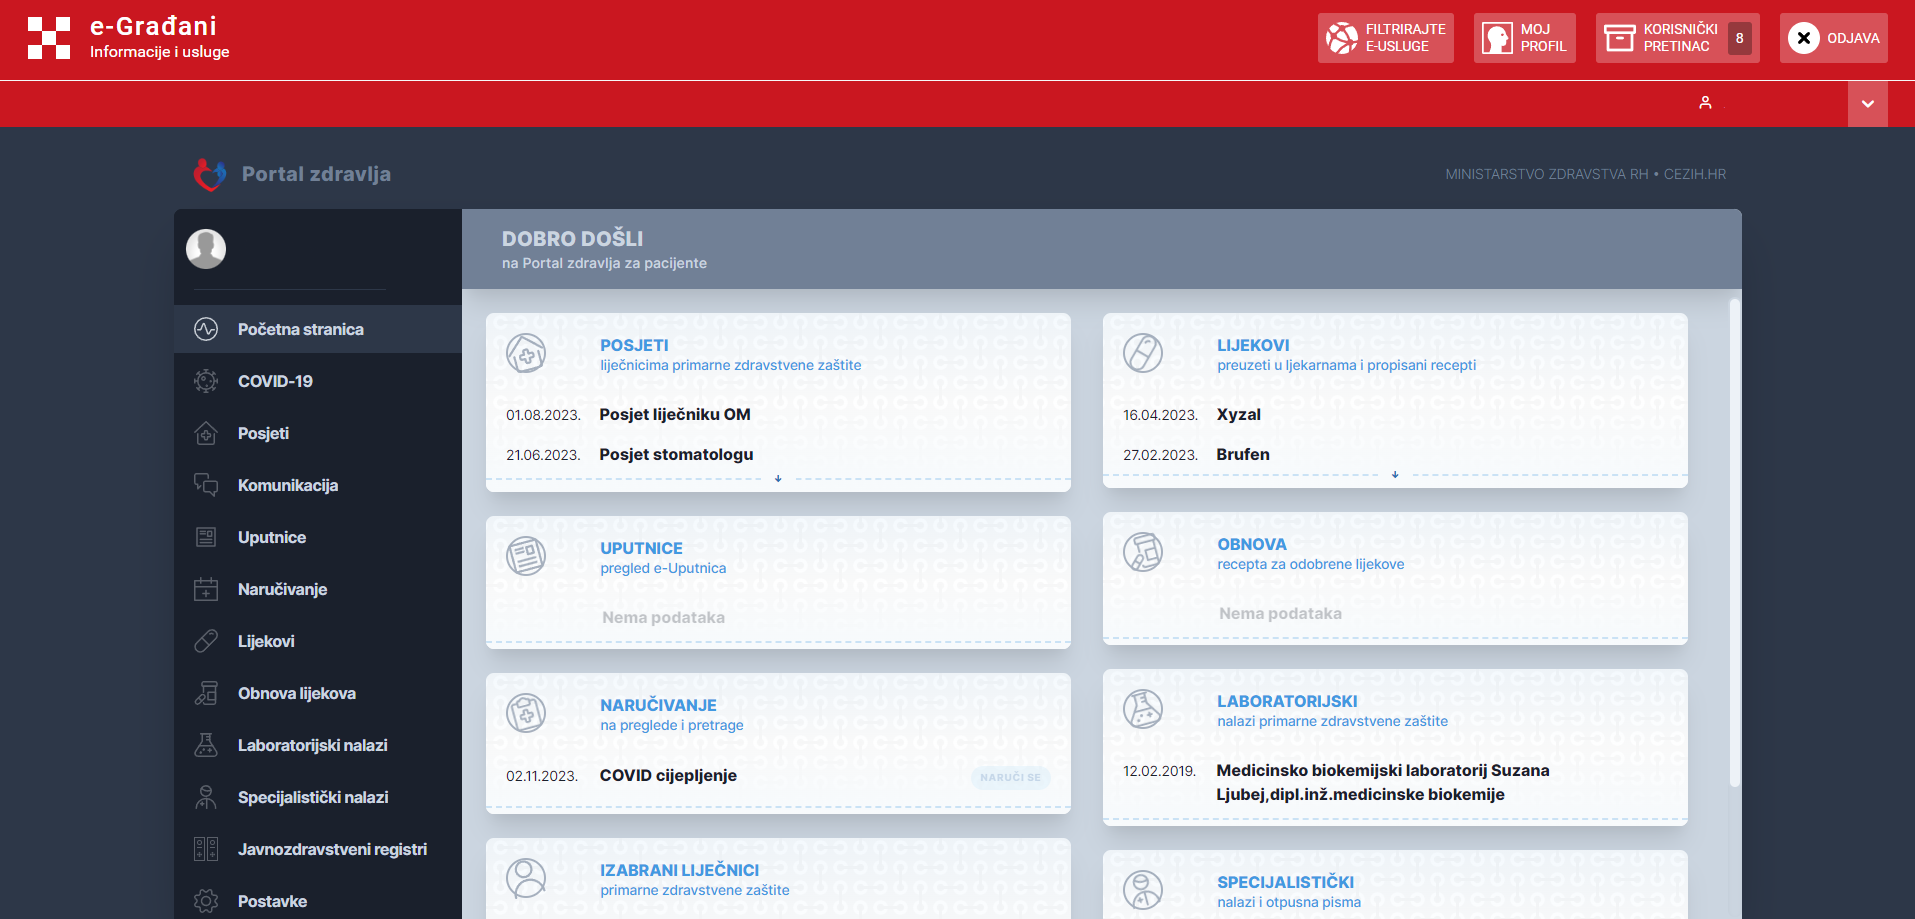
\includegraphics[scale=0.4]{slike/portalzdravlje.PNG} %veličina slike u odnosu na originalnu datoteku i pozicija slike
			\centering
			\caption{Izgled početnog izbornika platforme \textit{Portal zdravlja}}
			\label{fig:portal-zdravlja}
		\end{figure}
		
		\section{Opseg i prilagodljivost projektnog zadatka}
		Opisan rad aplikacije ostvaren je korištenjem nekoliko alata. Najprije, za razvoj \textit{backend-a} koristili smo alat \textit{Spring Boot}, gdje smo programirali u programskom jeziku Java. Za bazu podataka koristili smo \textit{H2} koji je također prilagođen radu u Javi, a za razvoj \textit{frontend-a} koristili smo \textit{React}, biblioteku programskog jezika JavaScript. \\
		Aplikacija (prilagodljivost-dodati).
		
		
		\section{Primjeri u \LaTeX u}
		
		\textit{Ovo potpoglavlje izbrisati.}\\

		U nastavku se nalaze različiti primjeri kako koristiti osnovne funkcionalnosti \LaTeX a koje su potrebne za izradu dokumentacije. Za dodatnu pomoć obratiti se asistentu na projektu ili potražiti upute na sljedećim web sjedištima:
		\begin{itemize}
			\item Upute za izradu diplomskog rada u \LaTeX u - \url{https://www.fer.unizg.hr/_download/repository/LaTeX-upute.pdf}
			\item \LaTeX\ projekt - \url{https://www.latex-project.org/help/}
			\item StackExchange za Tex - \url{https://tex.stackexchange.com/}\\
		
		\end{itemize} 	


		
		\noindent \underbar{podcrtani tekst}, \textbf{podebljani tekst}, 	\textit{nagnuti tekst}\\
		\noindent \normalsize primjer \large primjer \Large primjer \LARGE {primjer} \huge {primjer} \Huge primjer \normalsize
				
		\begin{packed_item}
			
			\item  primjer
			\item  primjer
			\item  primjer
			\item[] \begin{packed_enum}
				\item primjer
				\item[] \begin{packed_enum}
					\item[1.a] primjer
					\item[b] primjer
				\end{packed_enum}
				\item primjer
			\end{packed_enum}
			
		\end{packed_item}
		
		\noindent primjer url-a: \url{https://www.fer.unizg.hr/predmet/proinz/projekt}
		
		\noindent posebni znakovi: \# \$ \% \& \{ \} \_ 
		$|$ $<$ $>$ 
		\^{} 
		\~{} 
		$\backslash$ 
		
		
		\begin{longtblr}[
			label=none,
			entry=none
			]{
				width = \textwidth,
				colspec={|X[8,l]|X[8, l]|X[16, l]|}, 
				rowhead = 1,
			} %definicija širine tablice, širine stupaca, poravnanje i broja redaka naslova tablice
			\hline \SetCell[c=3]{c}{\textbf{naslov unutar tablice}}	 \\ \hline[3pt]
			\SetCell{LightGreen}IDKorisnik & INT	&  	Lorem ipsum dolor sit amet, consectetur adipiscing elit, sed do eiusmod  	\\ \hline
			korisnickoIme	& VARCHAR &   	\\ \hline 
			email & VARCHAR &   \\ \hline 
			ime & VARCHAR	&  		\\ \hline 
			\SetCell{LightBlue} primjer	& VARCHAR &   	\\ \hline 
		\end{longtblr}
		

		\begin{longtblr}[
				caption = {Naslov s referencom izvan tablice},
				entry = {Short Caption},
			]{
				width = \textwidth, 
				colspec = {|X[8,l]|X[8,l]|X[16,l]|}, 
				rowhead = 1,
			}
			\hline
			\SetCell{LightGreen}IDKorisnik & INT	&  	Lorem ipsum dolor sit amet, consectetur adipiscing elit, sed do eiusmod  	\\ \hline
			korisnickoIme	& VARCHAR &   	\\ \hline 
			email & VARCHAR &   \\ \hline 
			ime & VARCHAR	&  		\\ \hline 
			\SetCell{LightBlue} primjer	& VARCHAR &   	\\ \hline 
		\end{longtblr}
	


		
		
		%unos slike
		\begin{figure}[H]
			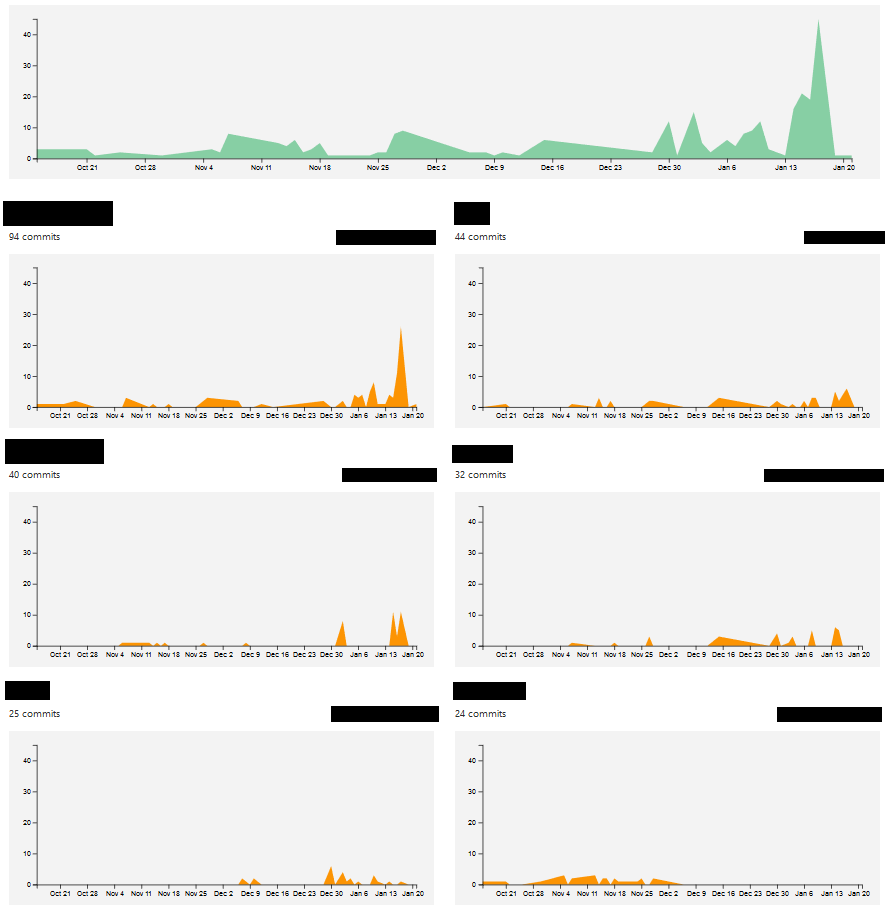
\includegraphics[scale=0.4]{slike/aktivnost.PNG} %veličina slike u odnosu na originalnu datoteku i pozicija slike
			\centering
			\caption{Izgled početnog izbornika platforme \textit{Portal zdravlja}}
			\label{fig:portal-zdravlja}
		\end{figure}
		
		\begin{figure}[H]
			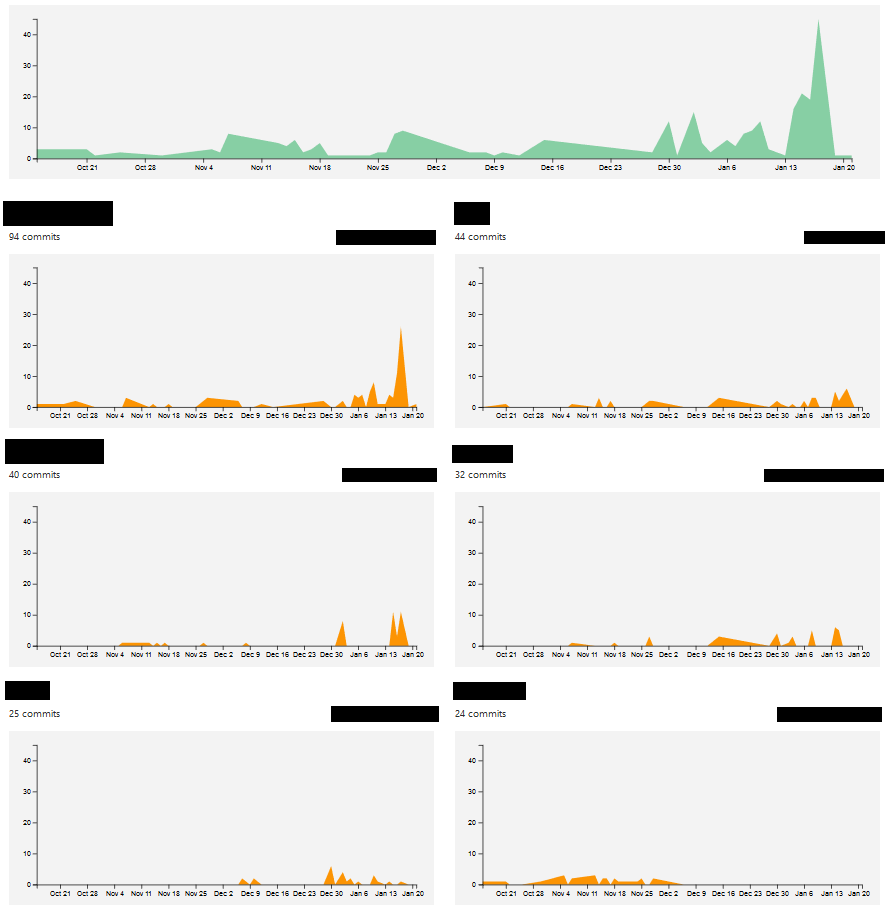
\includegraphics[width=\textwidth]{slike/aktivnost.PNG} %veličina u odnosu na širinu linije
			\caption{Primjer slike s potpisom 2}
			\label{fig:promjene2} %label mora biti drugaciji za svaku sliku
		\end{figure}
		
		Referenciranje slike \ref{fig:promjene2} u tekstu.
		
		\eject
		
	